\chapter{对比实验}
在之前的章节中,对本文提出的轨迹替换、混合高斯噪声层和仿真时间奖励等方法进行了初步实验验证。本章将通过严格控制变量的对比实验来进一步研究提出部分方法的有效性。

\section{混合高斯噪声层对比实验}
在混合高斯噪声层的对比实验中,除了在实验组的演员网络$\mu$添加了混合高斯噪声层以外,其余的算法参数均被设置为相同的数值。详细实验参数见表\ref{fcncmp}。其中各个实验参数的符号含义与上一章中的参数表\ref{simtable}含义相同。
    \begin{table}[htbp]
        \caption{混合高斯噪声层对比实验中的实验组与对照组}
        \label{fcncmp}
    \vspace{0.5em}\centering\wuhao
    \begin{tabular}{ccccc}
    \toprule[1.5pt]
        实验参数 & 实验组 & 对照组\\
    \midrule[1pt]
        $\sigma_{clip}$         & 0.5               & 0.5               \\
        $M$                     & 300               & 300               \\
        $\epsilon_{rand}$       & 0.3               & 0.3               \\
        $\xi_{action}$          & $1\times 10^{-3}$ & $1\times 10^{-3}$ \\
        $\gamma$                & 0.998             & 0.998             \\
        $\alpha$                & $1\times 10^{-3}$ & $1\times 10^{-3}$ \\
        $B$                     & 10000             & 10000             \\
        $\tau$                  & 0.23              & 0.23              \\
        $T$                     & 200               & 200               \\
        $N_{batches}$           & 1                 & 1                 \\
        $f_{target}$            & 200               & 200               \\
        $f_{actor}$             & 400               & 400               \\
        $f_{critic}$            & 200               & 200               \\
        $T_{start}$             & $1\times 10^5$    & $1\times 10^5$    \\
        $N_{sample}$            & 10                & 10                \\
        $k$                     & 18                & 18                \\
        $K_{replay}$            & 4                 & 4                 \\
        $\xi_{LSH}$             & $2\times 10^{-2}$ & $2\times 10^{-2}$ \\
        $\xi_{sim}$             & 0                 & 0                 \\
        是否使用混合高斯噪声层  & 是                & 否                \\
    \bottomrule[1.5pt]
    \end{tabular}
    \end{table}

添加了混合高斯噪声层的实验组与未添加混合高斯噪声层的对照组的演员网络损失曲线如图\ref{cmp1lossmu}所示。观察损失曲线可以发现,表示实验组的红色曲线上升到了更低的值并下降到了更低的值,这表明混合高斯噪声层可以增加训练过程的稳定性,减少损失发散的可能性。

        \begin{figure}[htpb]
        \centering
        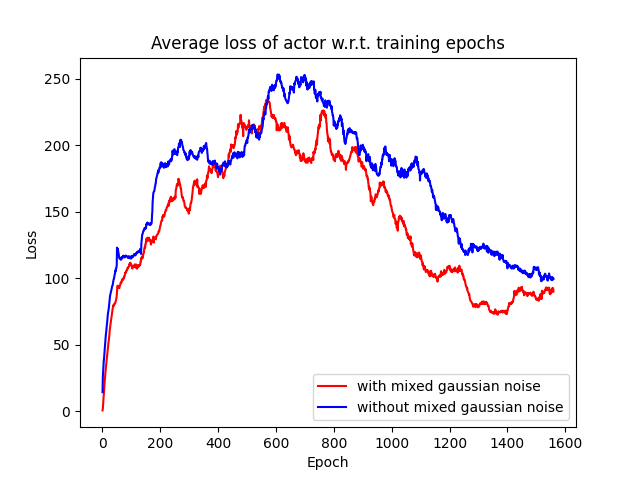
\includegraphics[width=0.6\textwidth]{compare1_lossmu.png}
        \caption{实验组与对照组演员网络$\mu$的损失曲线}
            \label{cmp1lossmu}
        \end{figure}

对于添加混合高斯噪声层的实验组和对照组的评论家网络的损失,如图\ref{cmp1lossq1}和\ref{cmp1lossq2}所示,变化趋势与演员网络类似。从图中可以看出,添加了混合高斯噪声层的实验组评论家网络损失没有像对照组那样出现大量尖峰,这意味着实验组的训练过程要比对照组更稳定。与此同时,实验组的两个评论家网络的损失大部分时间都要比对照组的损失略低,这也像演员网络损失曲线一样表明添加混合高斯噪声层的实验组智能体更不容易在训练过程中发散。
        \begin{figure}[htpb]
        \centering
        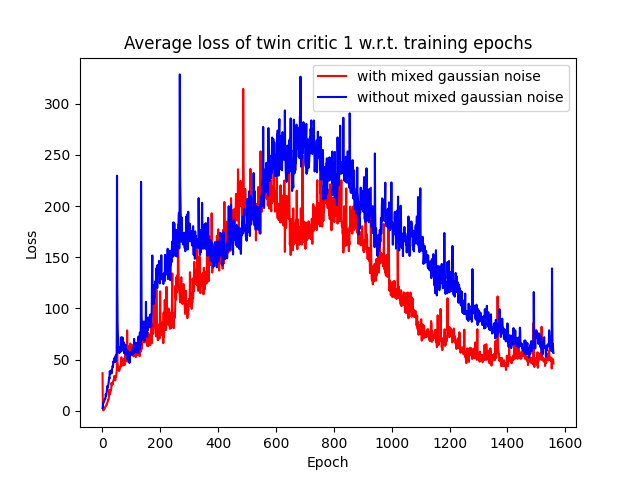
\includegraphics[width=0.6\textwidth]{compare1_lossq1.png}
        \caption{实验组与对照组评论家网络$Q_1$的损失曲线}
            \label{cmp1lossq1}
        \end{figure}

        \begin{figure}[htpb]
        \centering
        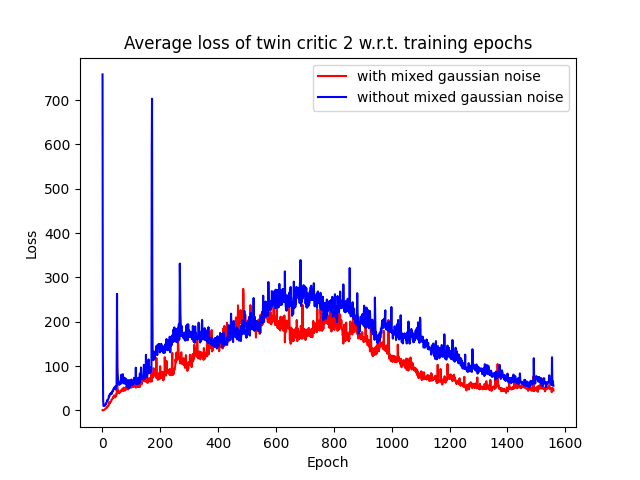
\includegraphics[width=0.6\textwidth]{compare1_lossq2.png}
        \caption{实验组与对照组评论家网络$Q_2$的损失曲线}
            \label{cmp1lossq2}
        \end{figure}

图\ref{cmp1env_reward}是添加了混合高斯噪声层的实验组和对照组在一代(10个片段)内的平均环境奖励。观察两个曲线可以发现,实验组在1200代时已经收敛到了比较高的平均环境奖励值,而对照组的平均环境奖励上升更慢且比实验组的奖励值更低。这表明添加了混合高斯噪声层后,智能体在环境中探索并获得奖励的能力获得了显著的提升,这也意味着混合高斯噪声层确实能帮助智能体得到更强的探索能力。
但是如果观察图\ref{cmp1suc_rate},可以发现添加混合高斯噪声层后平均任务目标成功率没有明显优于未添加的对照组。
统计第1500至1560代的成功率,得到添加混合高斯噪声层后的平均成功率为39.8\%,未添加的对照组为42.8\%。
考虑到成功率的计算只考虑了每个片段最后一个状态,而添加混合高斯噪声层后,智能体输出的动作受噪声影响,更有可能导致最后一个状态偏离目标,因此混合高斯噪声层在成功率上并不能显示出它的优势。
如果统计1500至1560代的平均奖励,可以得到添加混合高斯噪声层后,智能体获得的平均奖励为-146.0,而未添加的对照组为-150.7,这表明添加混合高斯噪声层后智能体获取奖励的能力更强。
        \begin{figure}[htpb]
        \centering
        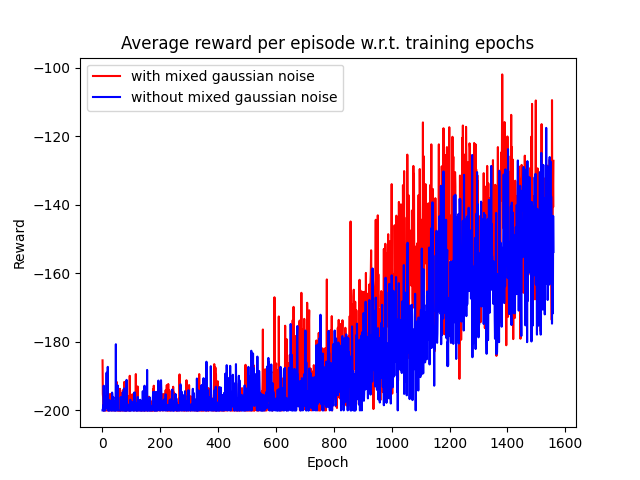
\includegraphics[width=0.6\textwidth]{compare1_reward.png}
        \caption{实验组和对照组的平均环境奖励曲线}
            \label{cmp1env_reward}
        \end{figure}

        \begin{figure}[htpb]
        \centering
        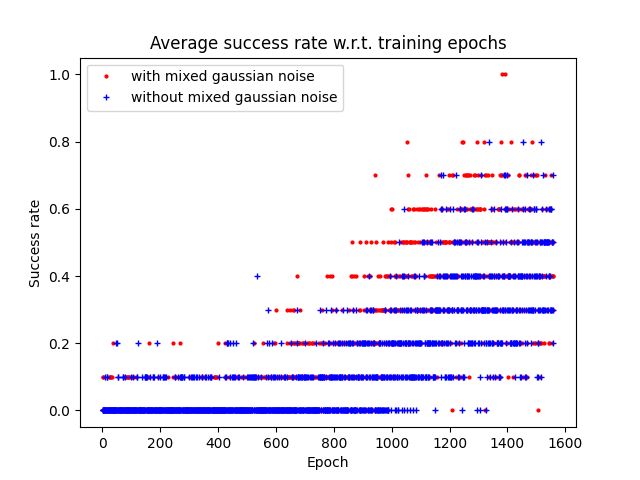
\includegraphics[width=0.6\textwidth]{compare1_suc_rate.png}
        \caption{实验组和对照组的平均任务目标成功率曲线}
            \label{cmp1suc_rate}
        \end{figure}

两组实验的基于局部敏感哈希的平均计数奖励曲线如图\ref{cmp1lsh_reward}所示。图中表示实验组的红色曲线在大部分时间都位于表示对照组的蓝色曲线上方。而基于局部敏感哈希的计数奖励表示了智能体探索到更不常见状态的多少,这表明添加混合高斯噪声层后,智能体更经常访问不常见的状态,从而导致了更多的奖励。因此添加了混合高斯噪声层可以改善智能体的探索策略,使之更偏向于访问更新奇的状态。
        \begin{figure}[htpb]
        \centering
        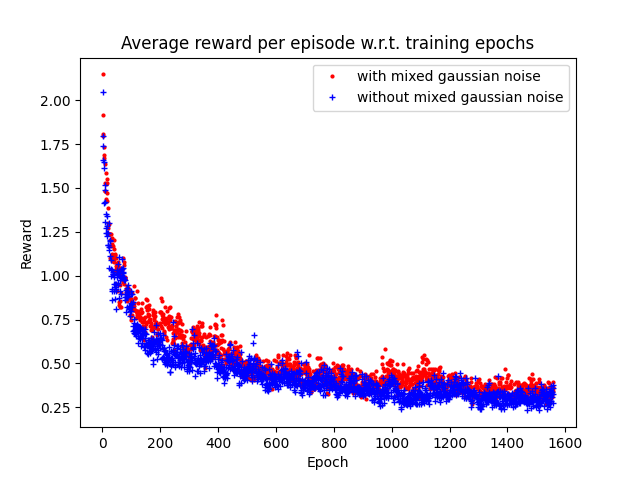
\includegraphics[width=0.6\textwidth]{compare1_lsh_reward.png}
        \caption{实验组和对照组的基于局部敏感哈希的平均计数奖励曲线}
            \label{cmp1lsh_reward}
        \end{figure}

\section{内部奖励的对比实验}

在上一章中的实验里,既使用了基于局部敏感哈希的计数奖励,又使用了仿真时间奖励,因此无法对比两种方法。因此在本节的对比实验中,除了实验组使用的内部奖励为仿真时间奖励,对照组使用的内部奖励为基于局部敏感哈希的计数奖励外,其余参数均保持相同。详细实验参数见表\ref{simcmp}。
    \begin{table}[htbp]
        \caption{内部奖励对比实验中的实验组与对照组}
        \label{simcmp}
    \vspace{0.5em}\centering\wuhao
    \begin{tabular}{ccccc}
    \toprule[1.5pt]
        实验参数 & 实验组 & 对照组\\
    \midrule[1pt]
        $\sigma_{clip}$         & 0.5               & 0.5               \\
        $M$                     & 300               & 300               \\
        $\epsilon_{rand}$       & 0.3               & 0.3               \\
        $\xi_{action}$          & $1\times 10^{-3}$ & $1\times 10^{-3}$ \\
        $\gamma$                & 0.998             & 0.998             \\
        $\alpha$                & $1\times 10^{-3}$ & $1\times 10^{-3}$ \\
        $B$                     & 10000             & 10000             \\
        $\tau$                  & 0.23              & 0.23              \\
        $T$                     & 200               & 200               \\
        $N_{batches}$           & 1                 & 1                 \\
        $f_{target}$            & 200               & 200               \\
        $f_{actor}$             & 400               & 400               \\
        $f_{critic}$            & 200               & 200               \\
        $T_{start}$             & $1\times 10^5$    & $1\times 10^5$    \\
        $N_{sample}$            & 10                & 10                \\
        $k$                     & 18                & 18                \\
        $K_{replay}$            & 4                 & 4                 \\
        $\xi_{LSH}$             & 0                 & $2\times 10^{-2}$ \\
        $\xi_{sim}$             & 10                & 0                 \\
        是否使用混合高斯噪声层  & 是                & 是                \\
    \bottomrule[1.5pt]
    \end{tabular}
    \end{table}
使用基于局部敏感哈希的计数奖励的对照组和使用仿真时间奖励的实验组的演员网络损失曲线如图\ref{cmp2lossmu}所示。可以看出表示实验组的蓝色曲线更快地下降到较低的损失值,这表示使用仿真时间奖励不会像基于局部敏感哈希的计数奖励那样由于奖励随时间变化更导致收敛速度变慢。

        \begin{figure}[htpb]
        \centering
        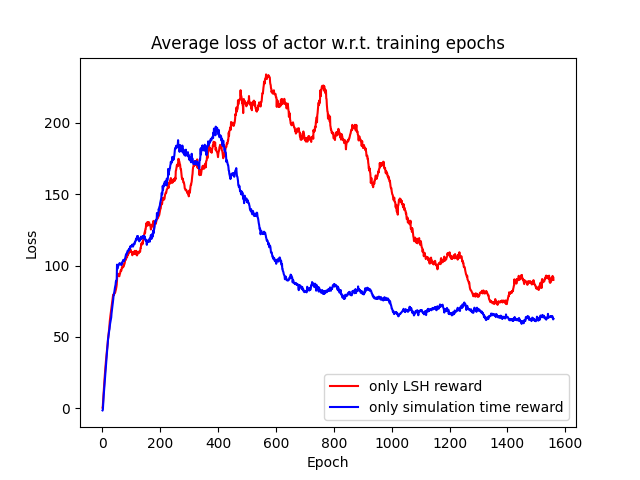
\includegraphics[width=0.6\textwidth]{compare2_lossmu.png}
        \caption{实验组与对照组演员网络$\mu$的损失曲线}
            \label{cmp2lossmu}
        \end{figure}

如图\ref{cmp2lossq1}和图\ref{cmp2lossq2}所示是实验组和对照组的评论家网络损失曲线。在两个图中除了训练刚开始时以外,都没有较为剧烈的尖峰,这表明改变内部奖励不会引起训练的不稳定性变化。此外,蓝色曲线也和演员网络损失曲线中一样更快地下降,这表明仿真时间奖励的训练过程要更快。

        \begin{figure}[htpb]
        \centering
        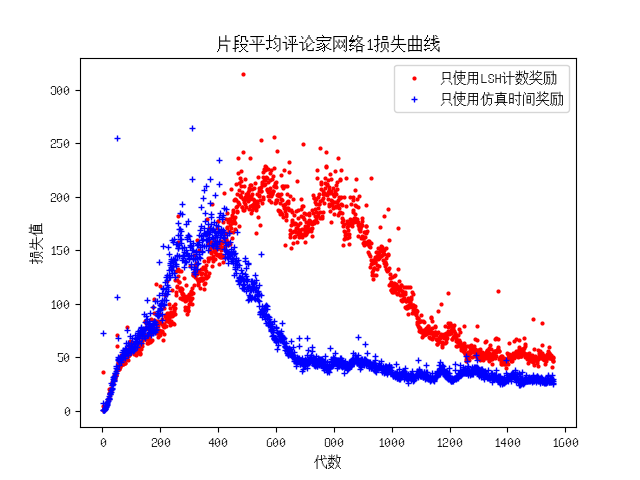
\includegraphics[width=0.6\textwidth]{compare2_lossq1.png}
        \caption{实验组与对照组评论家网络$Q_1$的损失曲线}
            \label{cmp2lossq1}
        \end{figure}

        \begin{figure}[htpb]
        \centering
        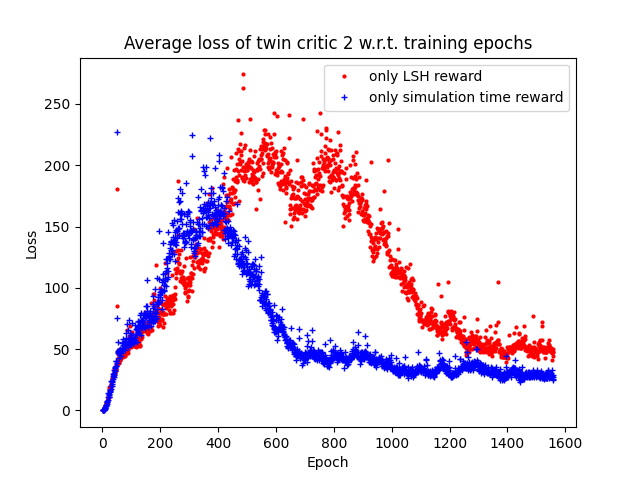
\includegraphics[width=0.6\textwidth]{compare2_lossq2.png}
        \caption{实验组与对照组评论家网络$Q_2$的损失曲线}
            \label{cmp2lossq2}
        \end{figure}

图\ref{cmp2env_reward}和图\ref{cmp2suc_rate}分别是平均环境奖励曲线和平均任务目标成功率曲线。在两个图中,蓝色曲线表示的仿真时间奖励都更快地收敛。
统计第1500代到1560代的成功率,可以得到只使用仿真时间奖励的平均成功率为48.3\%,只使用基于局部敏感哈希的计数奖励的平均成功率为42.8\%,因此使用仿真时间奖励可以比使用基于局部敏感哈希的计数奖励获得更高的成功率。
观察曲线也可以发现,在训练的大部分时间下,使用仿真时间奖励的智能体都获得了更高的环境奖励,达到了更高的任务成功率。
这表明仿真时间奖励要比基于局部敏感哈希的计数奖励能更有效地帮助智能体在环境中探索并在之后的开放任务中取得更好的成绩。
考虑到基于局部敏感哈希的计数奖励会在训练过程中逐渐衰减,因此重放缓冲中有可能对同样的迁移存放两个不同的计数奖励值,这会导致训练过程的不稳定,而仿真时间奖励没有这个问题,这可能是导致两种奖励出现性能差距的原因。
        \begin{figure}[htpb]
        \centering
        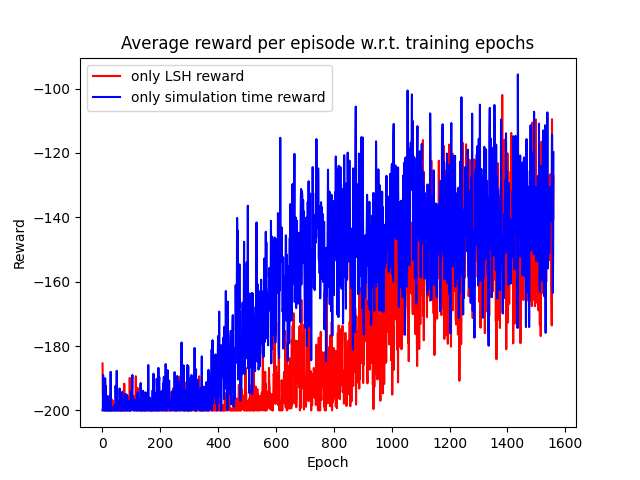
\includegraphics[width=0.6\textwidth]{compare2_reward.png}
        \caption{实验组和对照组的平均环境奖励曲线}
            \label{cmp2env_reward}
        \end{figure}

        \begin{figure}[htpb]
        \centering
        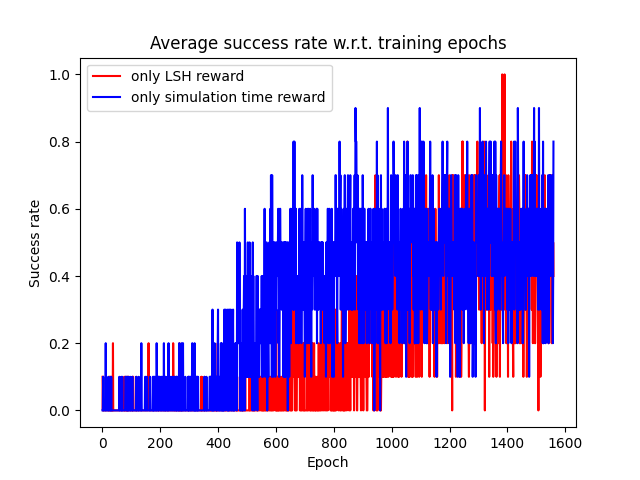
\includegraphics[width=0.6\textwidth]{compare2_suc_rate.png}
        \caption{实验组和对照组的平均任务目标成功率曲线}
            \label{cmp2suc_rate}
        \end{figure}
\section{本章小结}
本章通过添加混合高斯噪声层的智能体与未添加的进行对比,发现混合高斯噪声层能有效加速训练过程,提高探索效率。添加混合高斯噪声层后,训练过程中网络和损失的不稳定性也得到了控制,智能体获得了更高的平均环境奖励。

本章也对基于局部敏感哈希的计数奖励和仿真时间奖励进行了对比。实验结果表明仿真时间奖励显著优于基于局部敏感哈希的计数奖励。

        %\begin{figure}[htpb]
        %\centering
        %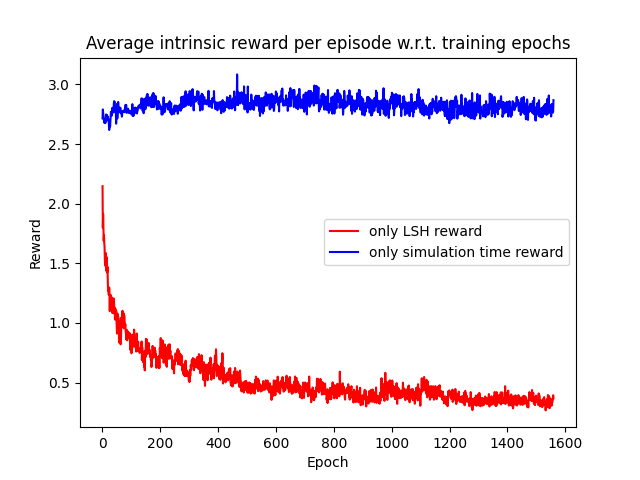
\includegraphics[width=0.6\textwidth]{compare2_in_reward.png}
        %\caption{实验组和对照组的平均内部奖励曲线}
        %    \label{cmp2in_reward}
        %\end{figure}
